\documentclass[11pt,a4paper]{article}

\usepackage[margin=1in]{geometry}
\usepackage{graphicx}
\usepackage{amsmath}
\usepackage{amssymb}
\usepackage{booktabs}
\usepackage{enumitem}
\usepackage{xcolor}
\usepackage{hyperref}
\usepackage{fancyhdr}
\usepackage{titlesec}
\usepackage{pdflscape}

% Colours matching the diagram palette
\definecolor{encblue}{HTML}{5a7fa0}
\definecolor{cvorange}{HTML}{c8861c}
\definecolor{refgreen}{HTML}{4a8a5f}
\definecolor{supred}{HTML}{c1121f}

\hypersetup{
  colorlinks=true,
  linkcolor=black,
  urlcolor=blue,
  citecolor=black,
}

\titleformat{\section}
  {\large\bfseries}{\thesection.}{0.5em}{}
\titleformat{\subsection}
  {\normalsize\bfseries}{\thesubsection}{0.5em}{}

\pagestyle{fancy}
\fancyhf{}
\rhead{\small StereoLite architecture}
\lhead{\small Nazib Abrar \textit{et al.}}
\cfoot{\thepage}

\title{\vspace{-1cm}\textbf{StereoLite: Architecture Document}}
\author{Nazib Abrar \quad Md Raihanul Haque Rahi \quad Md Zunaid Hossen \\
  \small{Department of Mechatronics Engineering, RUET}}
\date{\today}

\begin{document}
\maketitle
\thispagestyle{fancy}

\vspace{-0.5cm}

\begin{abstract}
\noindent
\textbf{StereoLite} is a lightweight stereo matching network targeted at
edge deployment (Jetson Orin Nano class hardware). It combines an
ImageNet-pretrained MobileNetV2 encoder, HITNet-style tile-hypothesis
representation, RAFT-style recurrent refinement, and a learned convex
upsampling head to produce dense disparity at full resolution. The model
totals \textbf{0.87\,M trainable parameters} and runs in
\textbf{54\,ms per 512$\times$832 pair on an RTX 3050}, with a validation
EPE of 1.62\,px on the Scene Flow Driving subset. This document provides
(i) the architecture diagram, (ii) a technical specification of every
stage, and (iii) a plain-English walkthrough intended for readers
unfamiliar with deep stereo matching.
\end{abstract}

% ======================================================================
\section{Architecture Diagram}
% ======================================================================

Figure~\ref{fig:arch} shows the complete StereoLite pipeline. Data flows
strictly left to right. Coloured blocks indicate three functional classes
of module: blue for the CNN encoder, orange for the cost volume and its
3D aggregator, and green for iterative refinement; grey denotes the
learned upsample. Small red dots along the top indicate where
supervision is applied.

\begin{figure*}[!htbp]
  \centering
  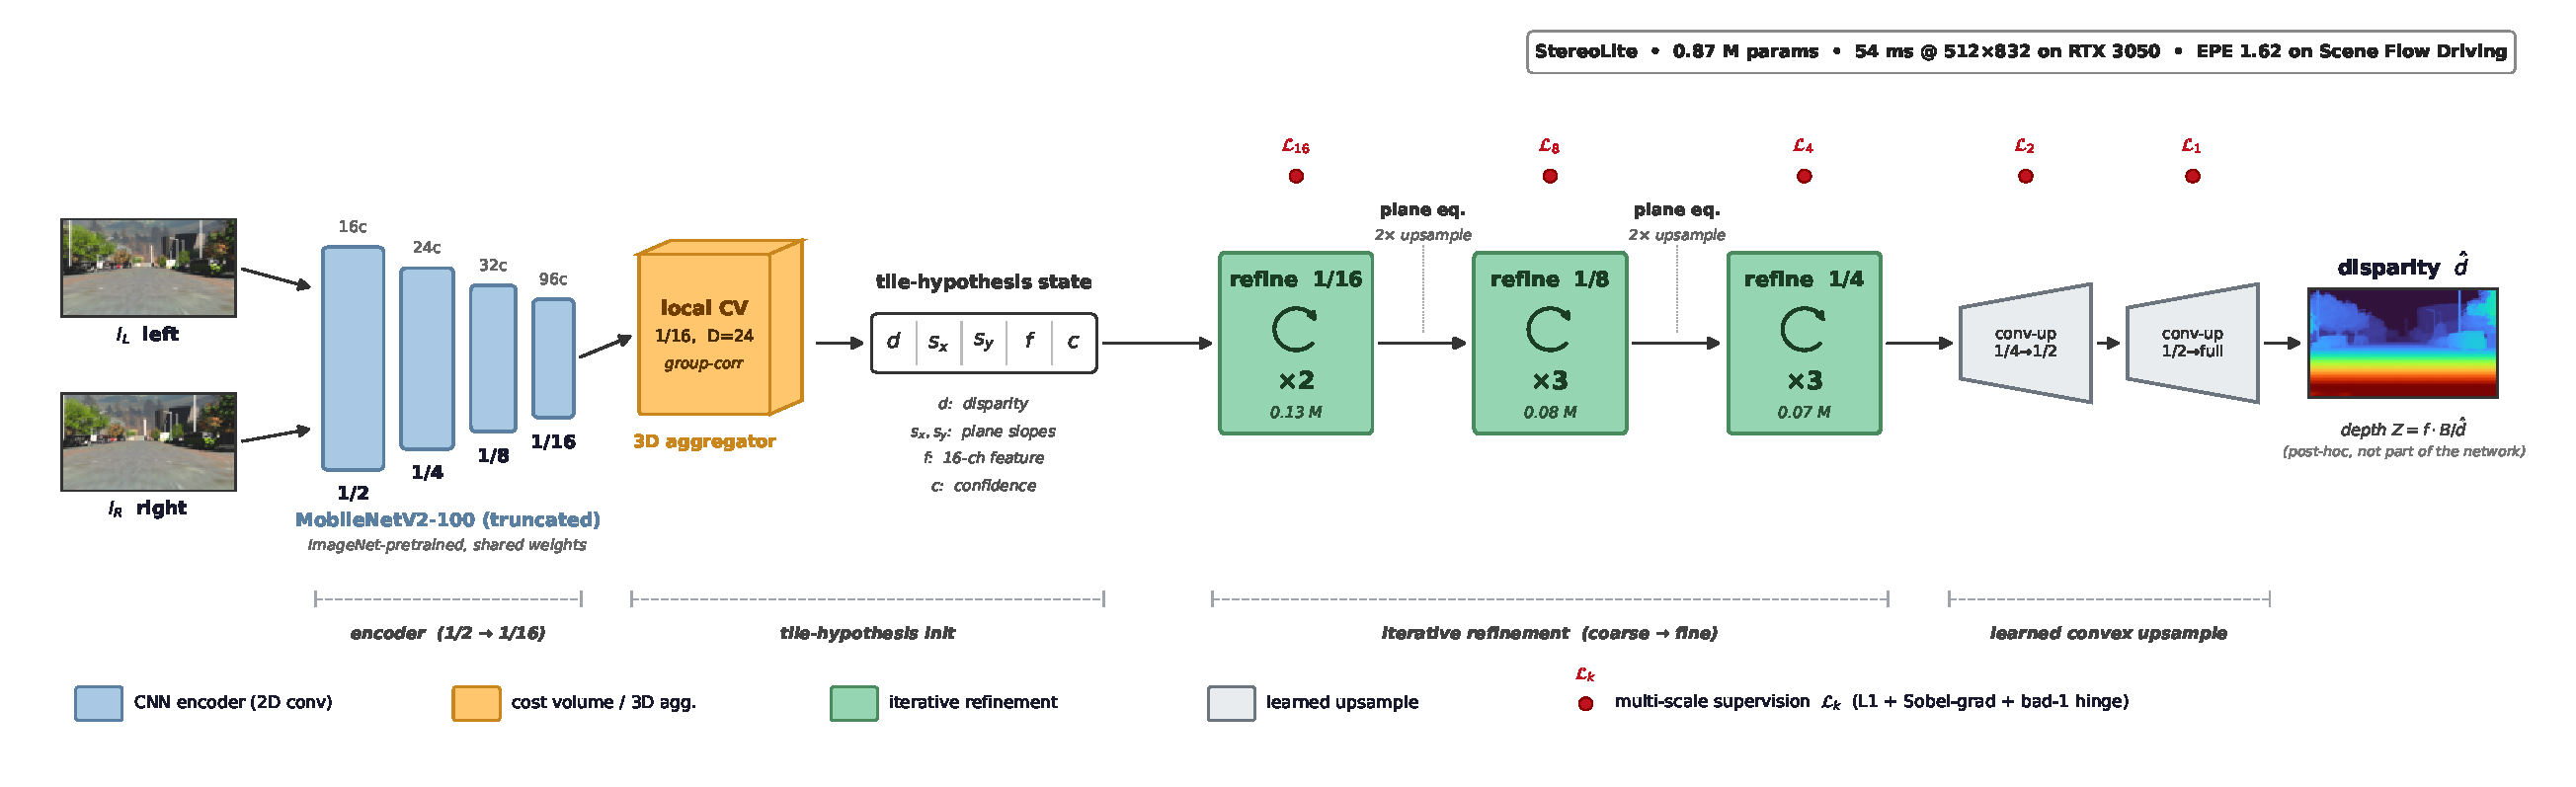
\includegraphics[width=\textwidth]{stereolite_arch.pdf}
  \caption{StereoLite end-to-end architecture. Input stereo pair on the
    left; predicted disparity $\hat{d}$ on the right. The model has four
    phases, labelled along the bottom rail: a truncated MobileNetV2-100
    encoder producing features at $\{1/2, 1/4, 1/8, 1/16\}$, a
    tile-hypothesis initialisation at $1/16$ using a group-correlation
    cost volume and a 3D aggregator, an iterative refinement stack that
    propagates and refines the tile state at $1/16$ ($\times 2$), $1/8$
    ($\times 3$), and $1/4$ ($\times 3$), and a learned convex-upsample
    cascade that produces the full-resolution disparity. Depth in
    metres is computed post-hoc from disparity via
    $Z = f\cdot B / \hat{d}$ and is not part of the network.}
  \label{fig:arch}
\end{figure*}

% ======================================================================
\section{Technical Specification}
% ======================================================================

\subsection{Notation}
\begin{itemize}[leftmargin=*, topsep=0pt, itemsep=1pt]
  \item $I_L, I_R \in \mathbb{R}^{B\times 3\times H\times W}$: input stereo
    pair, pixel values in $[0, 255]$.
  \item $f_{L,k}, f_{R,k}$: encoder features at scale $1/k$ for left and
    right images, $k \in \{2, 4, 8, 16\}$.
  \item $\hat{d} \in \mathbb{R}^{B\times 1\times H\times W}$: predicted
    full-resolution disparity.
  \item Tile state at scale $1/k$: $\mathcal{T}_k = (d, s_x, s_y, f, c)$
    where $d$ is disparity in $1/k$-px units, $(s_x, s_y)$ are plane
    slopes, $f$ is a 16-channel learned feature, $c$ is a scalar
    confidence.
\end{itemize}

\subsection{Encoder}
Shared MobileNetV2-100 with weights initialised from ImageNet. We use
timm's \texttt{features\_only} API with \texttt{out\_indices=(0,1,2,3)}.
After construction we \textbf{truncate} the internal block sequence to
drop everything past the deepest requested stage; this removes the
$1/32$ blocks (blocks 5 and 6, about 1\,M unused parameters) that would
otherwise run forward with zero backward gradient and break DDP. Channel
counts per scale:
\[
  (1/2: 16\text{c},\;\; 1/4: 24\text{c},\;\; 1/8: 32\text{c},\;\; 1/16: 96\text{c}).
\]
Input normalisation $(x - \mu) / \sigma$ with ImageNet statistics is
applied inside the encoder module. The encoder is fine-tuned end to end
with the rest of the network.

\subsection{Tile-Hypothesis Initialisation}
At the coarsest $1/16$ scale we build a single \textbf{group-wise
correlation cost volume} with 8 groups and 24 disparity candidates. The
volume has shape $(B, 8, 24, H/16, W/16)$ and is normalised
per-group-per-disparity. A small 3D aggregator (two \texttt{Conv3d}
layers, \texttt{GroupNorm}, \texttt{SiLU}) produces a single-channel
logit volume; softmax across disparity followed by soft-argmin gives the
initial disparity $d_0$. Confidence $c_0$ is the peak softmax
probability. Slopes $s_x, s_y$ are initialised to zero. A single-layer
head on $f_{L,16}$ produces the initial 16-channel tile feature $f_0$.
The combined $\mathcal{T}_{16} = (d_0, 0, 0, f_0, c_0)$ is the starting
state for the refinement stack.

\subsection{Iterative Refinement}
Each scale $k \in \{16, 8, 4\}$ has its own \texttt{TileRefine} module
with independently learned weights. At scale $k$ the module is invoked
$N_k \in \{2, 3, 3\}$ times respectively. Each invocation:
\begin{enumerate}[leftmargin=*, topsep=2pt, itemsep=1pt]
  \item Warps $f_{R,k}$ by the current disparity $d$ using horizontal
    bilinear sampling (\texttt{F.grid\_sample}).
  \item Concatenates $[f_{L,k}, \text{warp}(f_{R,k}), f, d, s_x, s_y, c]$
    along the channel axis.
  \item Applies a three-layer convolutional trunk (3$\times$3,
    hidden$=$48, \texttt{GN}, \texttt{SiLU}) and five $1\times 1$ output
    heads predicting residuals $\Delta d$, $\Delta s_x$, $\Delta s_y$,
    $\Delta f$, and $\Delta c$.
  \item Updates the state:
    $d \leftarrow \mathrm{softplus}(d + \Delta d)$ (keeps it positive),
    $s_x \leftarrow s_x + 0.1\,\Delta s_x$,
    $s_y \leftarrow s_y + 0.1\,\Delta s_y$,
    $f \leftarrow f + \Delta f$,
    $c \leftarrow \sigma(2c - 1 + \Delta c)$.
\end{enumerate}

\subsection{Scale Transitions (Plane-equation Upsample)}
Between refinement scales we upsample the tile state via the plane
equation: each parent tile at position $(y, x)$ with disparity $d$ and
slopes $(s_x, s_y)$ spawns four child tiles at offsets
$(\pm 0.25, \pm 0.25)$ in parent units. Child disparity is
\[
  d_\text{child} = 2\,d_\text{parent}
    + (2\,s_x)\,\Delta x + (2\,s_y)\,\Delta y,
\]
where the factor of 2 rescales from parent-unit to child-unit
disparity and $(\Delta x, \Delta y) \in \{\pm 0.25, \pm 0.25\}$. Slopes,
features, and confidence are bilinearly upsampled. This keeps the
cost-volume construction confined to a single scale and obtains sub-pixel
accuracy via the learned slopes, rather than rebuilding a CV at every
finer scale.

\subsection{Convex Upsample Cascade}
The final $1/4$ disparity is brought to full resolution by two
\texttt{ConvexUpsample} blocks (RAFT-Stereo style): a learned mask
predicts a 9-neighbour softmax over each $2\times 2$ sub-pixel block, and
the fine disparity is the weighted average of the 9 coarse neighbours
scaled by the upsample factor. Masks are conditioned on the encoder
features at the destination scale ($f_{L,4}$ for $1/4 \rightarrow 1/2$,
$f_{L,2}$ for $1/2 \rightarrow \text{full}$). This yields sub-pixel
boundary sharpness without adding another cost-volume stage.

\subsection{Outputs and Depth Conversion}
The network predicts \textbf{disparity} $\hat{d}$ in pixels. Metric
depth $Z$ is a post-hoc geometric conversion using the calibrated
stereo pair's focal length $f$ and baseline $B$:
\[
  Z \;=\; \frac{f \cdot B}{\hat{d}}.
\]
No learned parameters are involved in this conversion; it is applied
outside the network.

\subsection{Supervision}
Multi-scale L1 is applied at every intermediate disparity output:
$d_{32}$ (tile init), $d_{16}$, $d_{8}$, $d_{4}$, $d_{1/2}$, $d_{1/1}$.
The full loss is
\[
  \mathcal{L} = \sum_{k} w_k \Bigl[
    \ell_1^{(k)}
    + \lambda_g\,\ell_\text{grad}^{(k)}
    + \lambda_h\,\ell_\text{hinge}^{(k)}
  \Bigr]
    + \lambda_s\,\ell_\text{smooth}(\hat{d}, I_L),
\]
where $\ell_1^{(k)}$ is the masked L1 on valid pixels,
$\ell_\text{grad}^{(k)}$ is an L1 on Sobel-$(x,y)$ gradients of the
disparity (preserves edges), $\ell_\text{hinge}^{(k)}$ is a bad-1 hinge
(penalises errors $> 1$\,px more aggressively), and
$\ell_\text{smooth}$ is an edge-aware smoothness term weighted by
$\exp(-|\nabla I_L|/\sigma)$. Defaults:
$\lambda_g = 0.5, \lambda_h = 0.3, \lambda_s = 0.02, \sigma = 3.0$;
scale weights $w_k = \{0.2, 1.0, 0.3, 0.5, 0.7, 1.0\}$.

\subsection{Training Recipe}
AdamW with weight decay $10^{-5}$, OneCycle LR schedule peaking at
$8\times 10^{-4}$ with 5\% warmup, mixed-precision (\texttt{fp16}) forward
with \texttt{GradScaler}. Data augmentation: horizontal random-erase on
the right image only ($p=0.3$, up to 2 patches of 2--10\% of image
area) to force robust correspondence.

\subsection{Parameter Budget}
\begin{center}
\begin{tabular}{lr}
\toprule
Component & Params \\
\midrule
MobileNetV2-100 encoder (truncated to 1/16) & 0.54\,M \\
Tile init (cost volume + 3D aggregator + feat head) & 0.03\,M \\
Refine 1/16 ($\times$2 iters) & 0.13\,M \\
Refine 1/8  ($\times$3 iters) & 0.08\,M \\
Refine 1/4  ($\times$3 iters) & 0.07\,M \\
Convex upsample 1/4$\rightarrow$1/2 & 0.01\,M \\
Convex upsample 1/2$\rightarrow$full & 0.01\,M \\
\midrule
\textbf{Total trainable} & \textbf{0.874\,M} \\
BatchNorm running stats (buffers) & 0.032\,M \\
\midrule
\textbf{Checkpoint size (fp32)} & \textbf{8.7\,MB} \\
\bottomrule
\end{tabular}
\end{center}

% ======================================================================
\clearpage
\section{Plain-English Walkthrough}
% ======================================================================

This section explains what every stage of the network does in ordinary
language, assuming the reader has no deep-learning background. If you
know what a convolutional neural network is, you can safely skim the
first two paragraphs.

\subsection{What is the network trying to do?}

Imagine two cameras mounted side by side, like your eyes. They see the
same scene, but from slightly different positions. Because of that, an
object close to the cameras \textit{shifts} between the two views more
than an object far away. The amount of shift, measured in pixels, is
called the \textbf{disparity}. Small disparity means far away; large
disparity means close.

Our network takes the two images as input and produces a disparity map
that tells us, for every pixel in the left image, how far that pixel
appeared to move in the right image. From disparity we can compute
actual distance in metres via a simple formula involving the camera's
focal length and the distance between the two cameras. The network
itself never sees metres; it only learns to predict disparity.

\subsection{Stage 1: Encoder (blue blocks)}

The two images first pass through the same feature extractor, a
compact CNN called \textbf{MobileNetV2}. This module was
originally trained on the ImageNet photo-classification task, so it
already knows how to recognise useful patterns like edges, corners,
textures, and object boundaries. We re-use those weights as our
starting point rather than training from scratch.

As the image flows through the encoder, it is progressively downsampled:
the first block outputs features at half resolution ($1/2$), the next at
$1/4$, then $1/8$, and finally $1/16$. At each stage the spatial
resolution shrinks and the number of descriptive channels grows. Think
of it as zooming out while also paying more attention to what each
region of the image ``means'' rather than just its raw pixels.

Because the same encoder processes both the left and right image, the
features are directly comparable between the two views, which is
essential for matching in the next stage.

\subsection{Stage 2: Tile-hypothesis initialisation (orange block)}

At the coarsest scale ($1/16$), the network does its first guess at
disparity using a \textbf{cost volume}. For every pixel in the left
feature map, we compare its feature vector to feature vectors of nearby
pixels in the right feature map at 24 different horizontal shifts. The
more similar they are, the lower the ``cost'' of that shift.

A tiny 3D CNN (the \emph{3D aggregator}) smooths this cost volume. Then
a soft-argmin operation picks the best shift for each pixel. This gives
us an initial, rough disparity map at $1/16$ scale.

Rather than just storing a single disparity number per tile, the network
packages it into a richer \textbf{tile hypothesis}: five quantities per
tile
\begin{itemize}[leftmargin=*, topsep=1pt, itemsep=0pt]
  \item $d$: the disparity value itself.
  \item $s_x$: how the disparity changes going right (the left-right
    slope of the underlying 3D surface).
  \item $s_y$: how the disparity changes going down (the up-down
    slope).
  \item $f$: a 16-number learned ``memory'' that the refinement stages
    can write into and read from.
  \item $c$: a confidence score in $[0, 1]$ saying how trustworthy this
    tile's disparity is.
\end{itemize}
Representing each tile as a slanted little plane, rather than a flat
patch, is a classic idea from the \textit{HITNet} paper. It lets the
network capture oriented surfaces like roads and walls gracefully.

\subsection{Stage 3: Iterative refinement (green blocks)}

This is the heart of the model. The coarse $1/16$ hypothesis is good
enough to point us in the right direction, but not accurate enough to be
the final answer. So we refine it in a \textbf{coarse-to-fine} schedule
over three scales:
\begin{enumerate}[leftmargin=*, topsep=1pt, itemsep=0pt]
  \item At $1/16$, run two refinement iterations.
  \item Upsample the tile state to $1/8$, run three iterations.
  \item Upsample to $1/4$, run three more iterations.
\end{enumerate}
Each iteration is the same recipe:
\begin{enumerate}[leftmargin=*, topsep=1pt, itemsep=0pt]
  \item Take the current disparity $d$ and use it to \emph{warp} the
    right feature map so that it (approximately) aligns with the left.
  \item Compare the warped right features to the left features.
  \item From that comparison, predict small \textbf{corrections} to all
    five state quantities: $\Delta d, \Delta s_x, \Delta s_y, \Delta f,
    \Delta c$.
  \item Add the corrections to the current state.
\end{enumerate}
This is the \textbf{RAFT} idea: instead of predicting the answer in one
shot, predict a small correction each step and apply it repeatedly. It
turns out this converges much more accurately than a single big
prediction.

\subsection{Scale transitions: plane-equation upsample}

When we go from $1/16$ to $1/8$, each coarse tile becomes four finer
tiles. The obvious thing would be to just bilinearly interpolate the
disparity, but that loses the slopes we worked so hard to learn.
Instead, we use the \textbf{plane equation}: each child tile's
disparity is the parent's disparity \emph{plus} a small correction
computed from the parent's slopes and the child's relative position.
The slopes themselves, plus features and confidence, are bilinearly
upsampled. Effectively: the coarse tile is a tilted patch, and the four
children inherit their disparity from where they sit on that tilted
patch.

\subsection{Stage 4: Learned convex upsample (grey blocks)}

By the time we finish the $1/4$ refinement stack, we have a very good
disparity at $1/4$ resolution. To get to full resolution we use
\textbf{convex upsampling}, another idea borrowed from RAFT. For every
fine pixel, the network predicts nine weights that sum to one, and the
fine disparity is the weighted average of nine neighbouring coarse
disparities. Because the weights are learned and can attend to edges in
the input image, the upsampling is much sharper than bilinear. We chain
two of these blocks: $1/4 \rightarrow 1/2$ and $1/2 \rightarrow
\text{full}$.

\subsection{Output: disparity and depth}

The model's output is a full-resolution \textbf{disparity} map. That's
what the network actually learns. To turn disparity into metric depth
we simply apply the pinhole formula
\[
  Z = \frac{f \cdot B}{\hat{d}}
\]
where $f$ is the focal length of the cameras in pixels, $B$ is the
horizontal distance between them in metres, and $\hat{d}$ is our
predicted disparity in pixels. This conversion is geometric and has no
learnable parameters.

\subsection{How we train it}

During training, for every pair of input images we know the true
disparity (either from ray-traced synthetic data or from LiDAR in
real-world data). We compare the network's predicted disparity to the
ground truth at \textbf{every scale}, not just the final output: the
tile-init at $1/32$, the refined outputs at $1/16$, $1/8$, $1/4$, and
the two upsampled outputs at $1/2$ and full. Supervising every
intermediate output (the red dots on the diagram) keeps the network
from collapsing into a single big end-to-end prediction and forces each
stage to contribute usefully.

We combine three losses:
\begin{itemize}[leftmargin=*, topsep=1pt, itemsep=0pt]
  \item $L_1$: the average absolute pixel error.
  \item Gradient: we apply a Sobel filter to both predicted and true
    disparity and penalise differences, which keeps edges sharp.
  \item Bad-1 hinge: pixels whose error is larger than 1\,px get an
    extra penalty, discouraging occasional large mistakes.
\end{itemize}
A separate edge-aware smoothness term encourages the full-resolution
disparity to be smooth in flat image regions (like roads and walls) but
allows sharp jumps at image edges.

The optimiser is AdamW; the learning rate follows a one-cycle schedule
peaking at $8\times 10^{-4}$. Training is mixed-precision (\texttt{fp16})
for speed.

\subsection{Why it is small and fast}

Every design decision in StereoLite trades accuracy against inference
cost:
\begin{itemize}[leftmargin=*, topsep=1pt, itemsep=0pt]
  \item We use a \textbf{single} cost volume at the \textbf{coarsest}
    scale instead of one per scale. That's where cost volumes are
    cheapest (fewest pixels) but still rich enough to initialise the
    refinement.
  \item We rely on \textbf{iterative refinement} rather than larger
    networks for accuracy.
  \item We \textbf{truncate} MobileNetV2 to the parts we actually use,
    removing about a million parameters of deep blocks whose features
    we never consume.
  \item The \textbf{convex upsample} cascade avoids a third cost volume
    at $1/2$ or full resolution.
\end{itemize}
The result is 0.87\,M trainable parameters and 54\,ms per 512$\times$832
pair on an RTX 3050 Laptop GPU. On a Jetson Orin Nano with INT8
quantisation we expect roughly $25$--$40$\,ms per pair, making real-time
stereo at 30\,fps feasible on an edge device.

\subsection{What the network does not do}

It is worth being explicit about what is \emph{not} happening inside
StereoLite:
\begin{itemize}[leftmargin=*, topsep=1pt, itemsep=0pt]
  \item It does not convert disparity to metric depth; that happens
    outside the network with known camera calibration.
  \item It does not do rectification; it assumes the left and right
    images are already row-aligned (standard stereo preprocessing).
  \item It does not produce confidence calibrated in any absolute
    sense; the confidence channel $c$ is a learned scalar used
    internally by the refinement stack, not a ground-truth-calibrated
    reliability estimate.
  \item It does not predict semantic segmentation, optical flow, or
    surface normals. Pure stereo disparity is the sole task.
\end{itemize}

% ======================================================================
\clearpage
\section{Training Results (Scene Flow Driving)}
% ======================================================================

This section reports the training run that produced the released
checkpoint. The model was trained on Kaggle T4$\times$2 with
DistributedDataParallel, batch~8 per GPU (effective batch~16), input
$512\!\times\!832$, OneCycle LR peaking at $8\!\times\!10^{-4}$, mixed
precision, and right-image random-erase augmentation (\(p=0.3\)).
30~epochs over 4{,}200 training pairs and 200 held-out val pairs from
Scene Flow Driving. Total wall-clock time on T4$\times$2: $\approx$
2\,h~10\,min.

\subsection{Final metrics}

\begin{center}
\begin{tabular}{lr}
\toprule
Metric & Value \\
\midrule
Validation EPE (200 held-out pairs) & \textbf{1.54\,px} \\
Validation bad-1 (\% pixels with $|\hat{d}-d^*|>1$\,px) & 25.2\,\% \\
Final training l1\_final & 1.40\,px \\
Final training l1\_cv (1/8 cost-volume head) & 0.13\,px \\
Total wall-clock (T4$\times$2) & $\approx$ 2\,h\,10\,min \\
Training steps completed & 7{,}850 \\
\bottomrule
\end{tabular}
\end{center}

\subsection{Training curves}

Figure~\ref{fig:curves} shows the training trajectory across all 7{,}850
steps. The total multi-scale loss (panel a) drops monotonically by two
orders of magnitude. The L1 errors on the final disparity (b) and on
the 1/8 cost-volume output (c) both converge cleanly without
overfitting; the gap between training and validation metrics
(VAL\,EPE\,$=$\,1.54 vs final training l1\_final\,$=$\,1.40) is small,
indicating reasonable generalisation on the held-out subset. The
OneCycle learning-rate schedule (d) ramps up linearly during the first
5\,\% of training and decays cosine-style for the remaining 95\,\%.

\begin{figure}[!htbp]
  \centering
  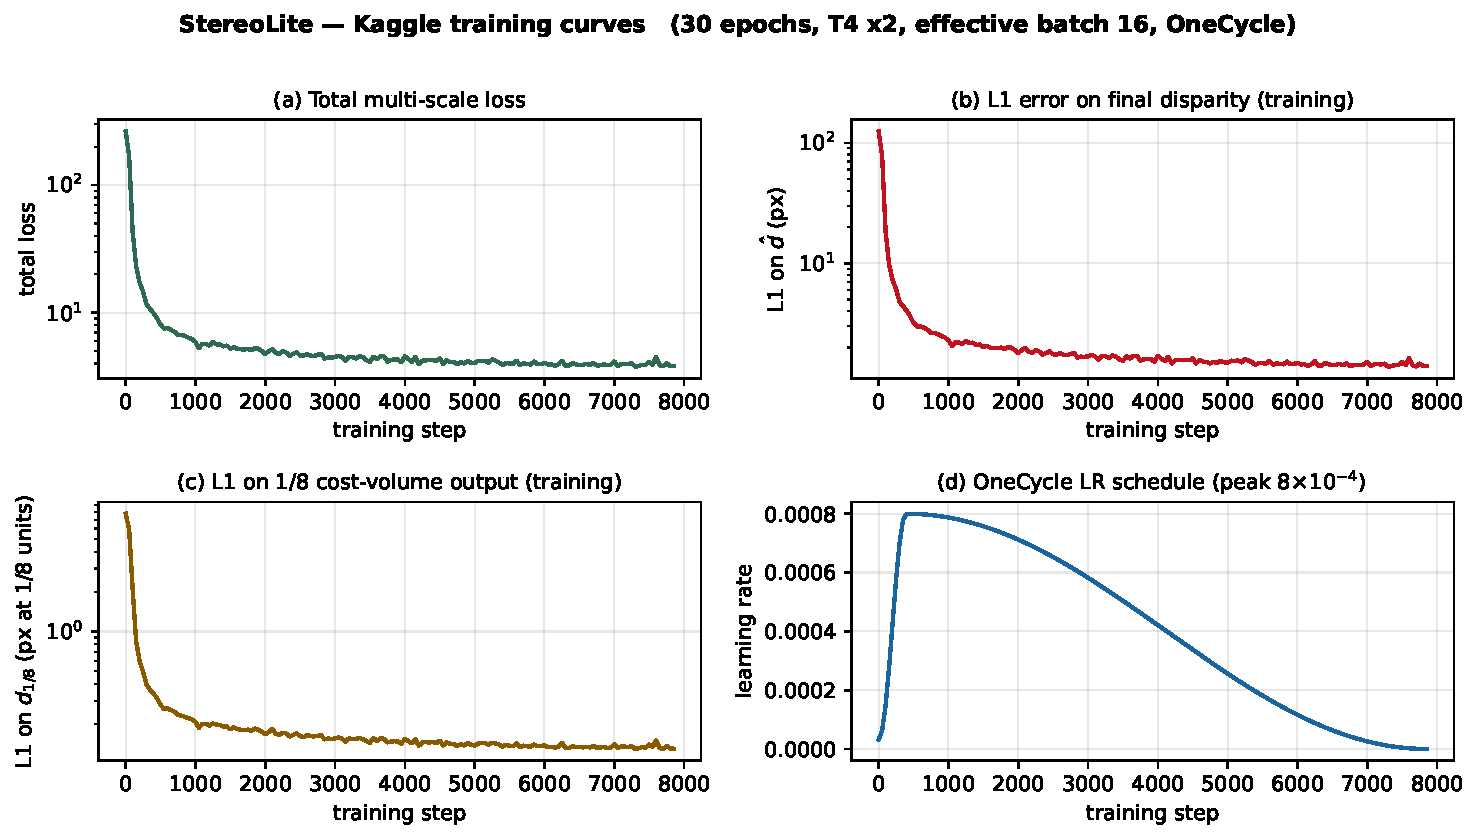
\includegraphics[width=\textwidth]{training_curves.pdf}
  \caption{Kaggle training curves over 30 epochs.
    (a)~total multi-scale loss (log scale);
    (b)~L1 on the full-resolution disparity;
    (c)~L1 on the 1/8 cost-volume output;
    (d)~OneCycle learning-rate schedule.}
  \label{fig:curves}
\end{figure}

\subsection{Per-step qualitative progression}

Figure~\ref{fig:progress} tracks two representative validation pairs
(a foliage-heavy scene with overlapping trees, and an urban scene with
a parked vehicle) across five training checkpoints from step~500 to
step~7500. The predicted disparity rapidly captures global scene
structure during the first 1{,}500 steps and gradually sharpens
foreground--background boundaries through the rest of training.

\begin{figure}[!htbp]
  \centering
  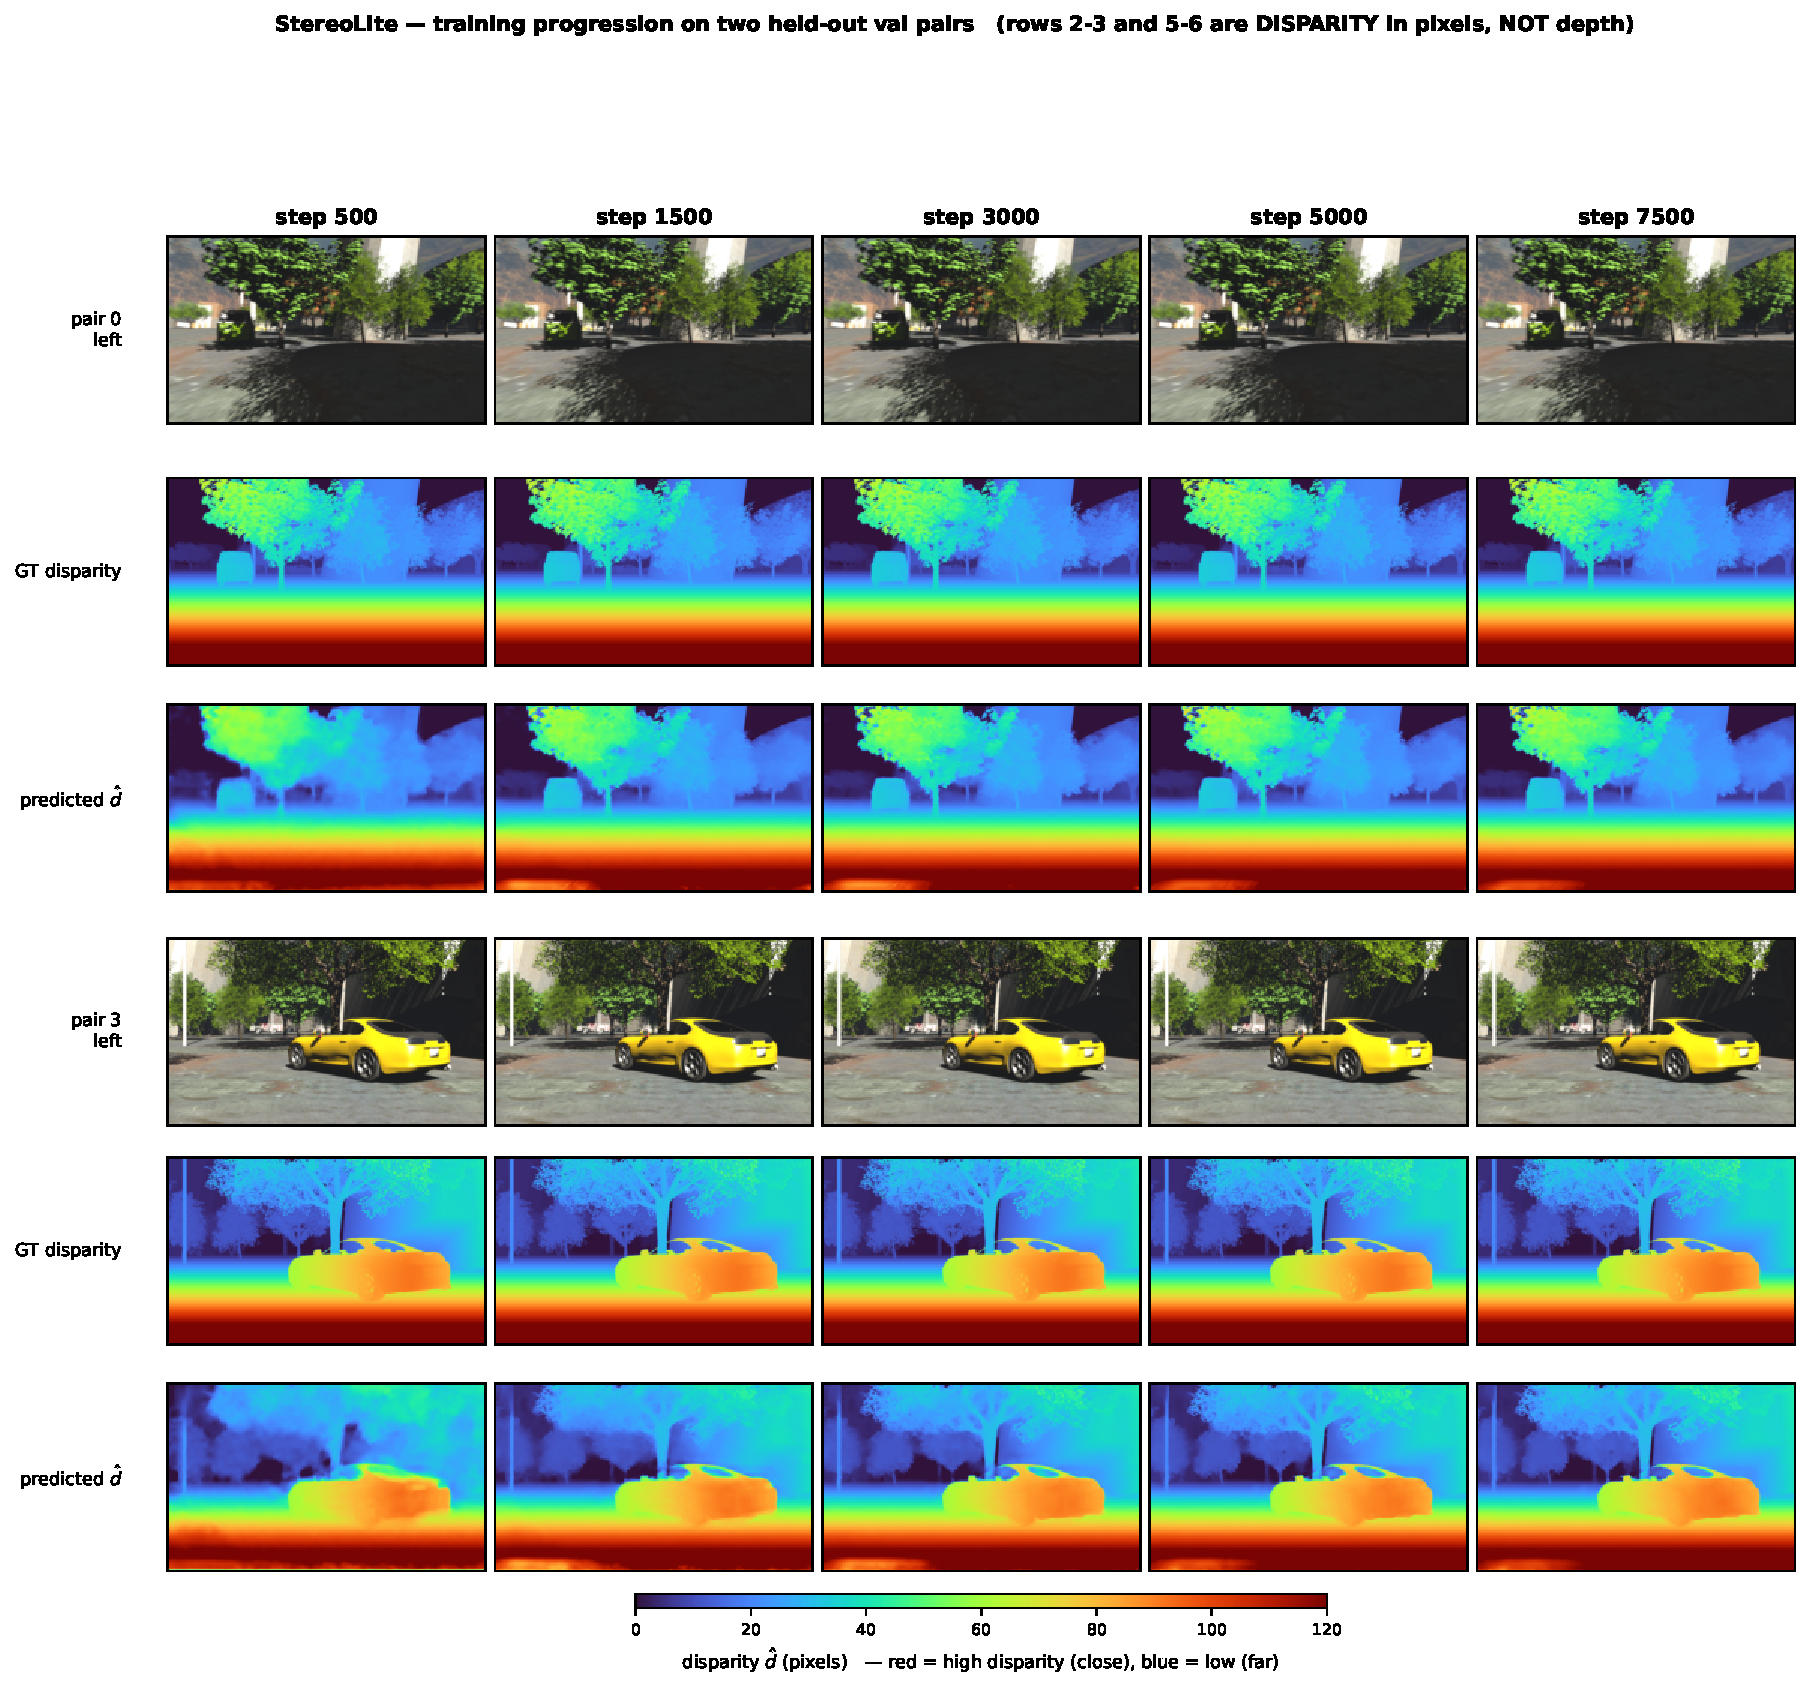
\includegraphics[width=\textwidth]{progress_grid.pdf}
  \caption{Training progression for two held-out validation pairs.
    Columns: training-step checkpoints. Rows for each pair: input left
    image $I_L$, ground-truth \textbf{disparity}, and predicted
    \textbf{disparity}~$\hat{d}$ (TURBO colourmap; red = high
    disparity / close, blue = low disparity / far). These are
    \emph{disparity} maps in pixel units, not depth maps in metres;
    metric depth would have the inverse colouring (blue = close, red =
    far) under the same colourmap.}
  \label{fig:progress}
\end{figure}

\subsection{Final-checkpoint gallery}

Figure~\ref{fig:gallery} shows all six tracked validation pairs at the
final step. The gallery covers the qualitative range of Scene Flow
Driving: foliage detail (pair 0), low-light/textureless regions (pair
1), highly slanted surfaces (pairs 2 and 4), foreground vehicles (pair
3), and reflective ground (pair 5). The model produces dense, sharply
delimited disparity maps across all of them, with the largest residual
errors (visible as colour-temperature mismatches) located where ground
truth is sparse along distant horizons.

\begin{figure}[!htbp]
  \centering
  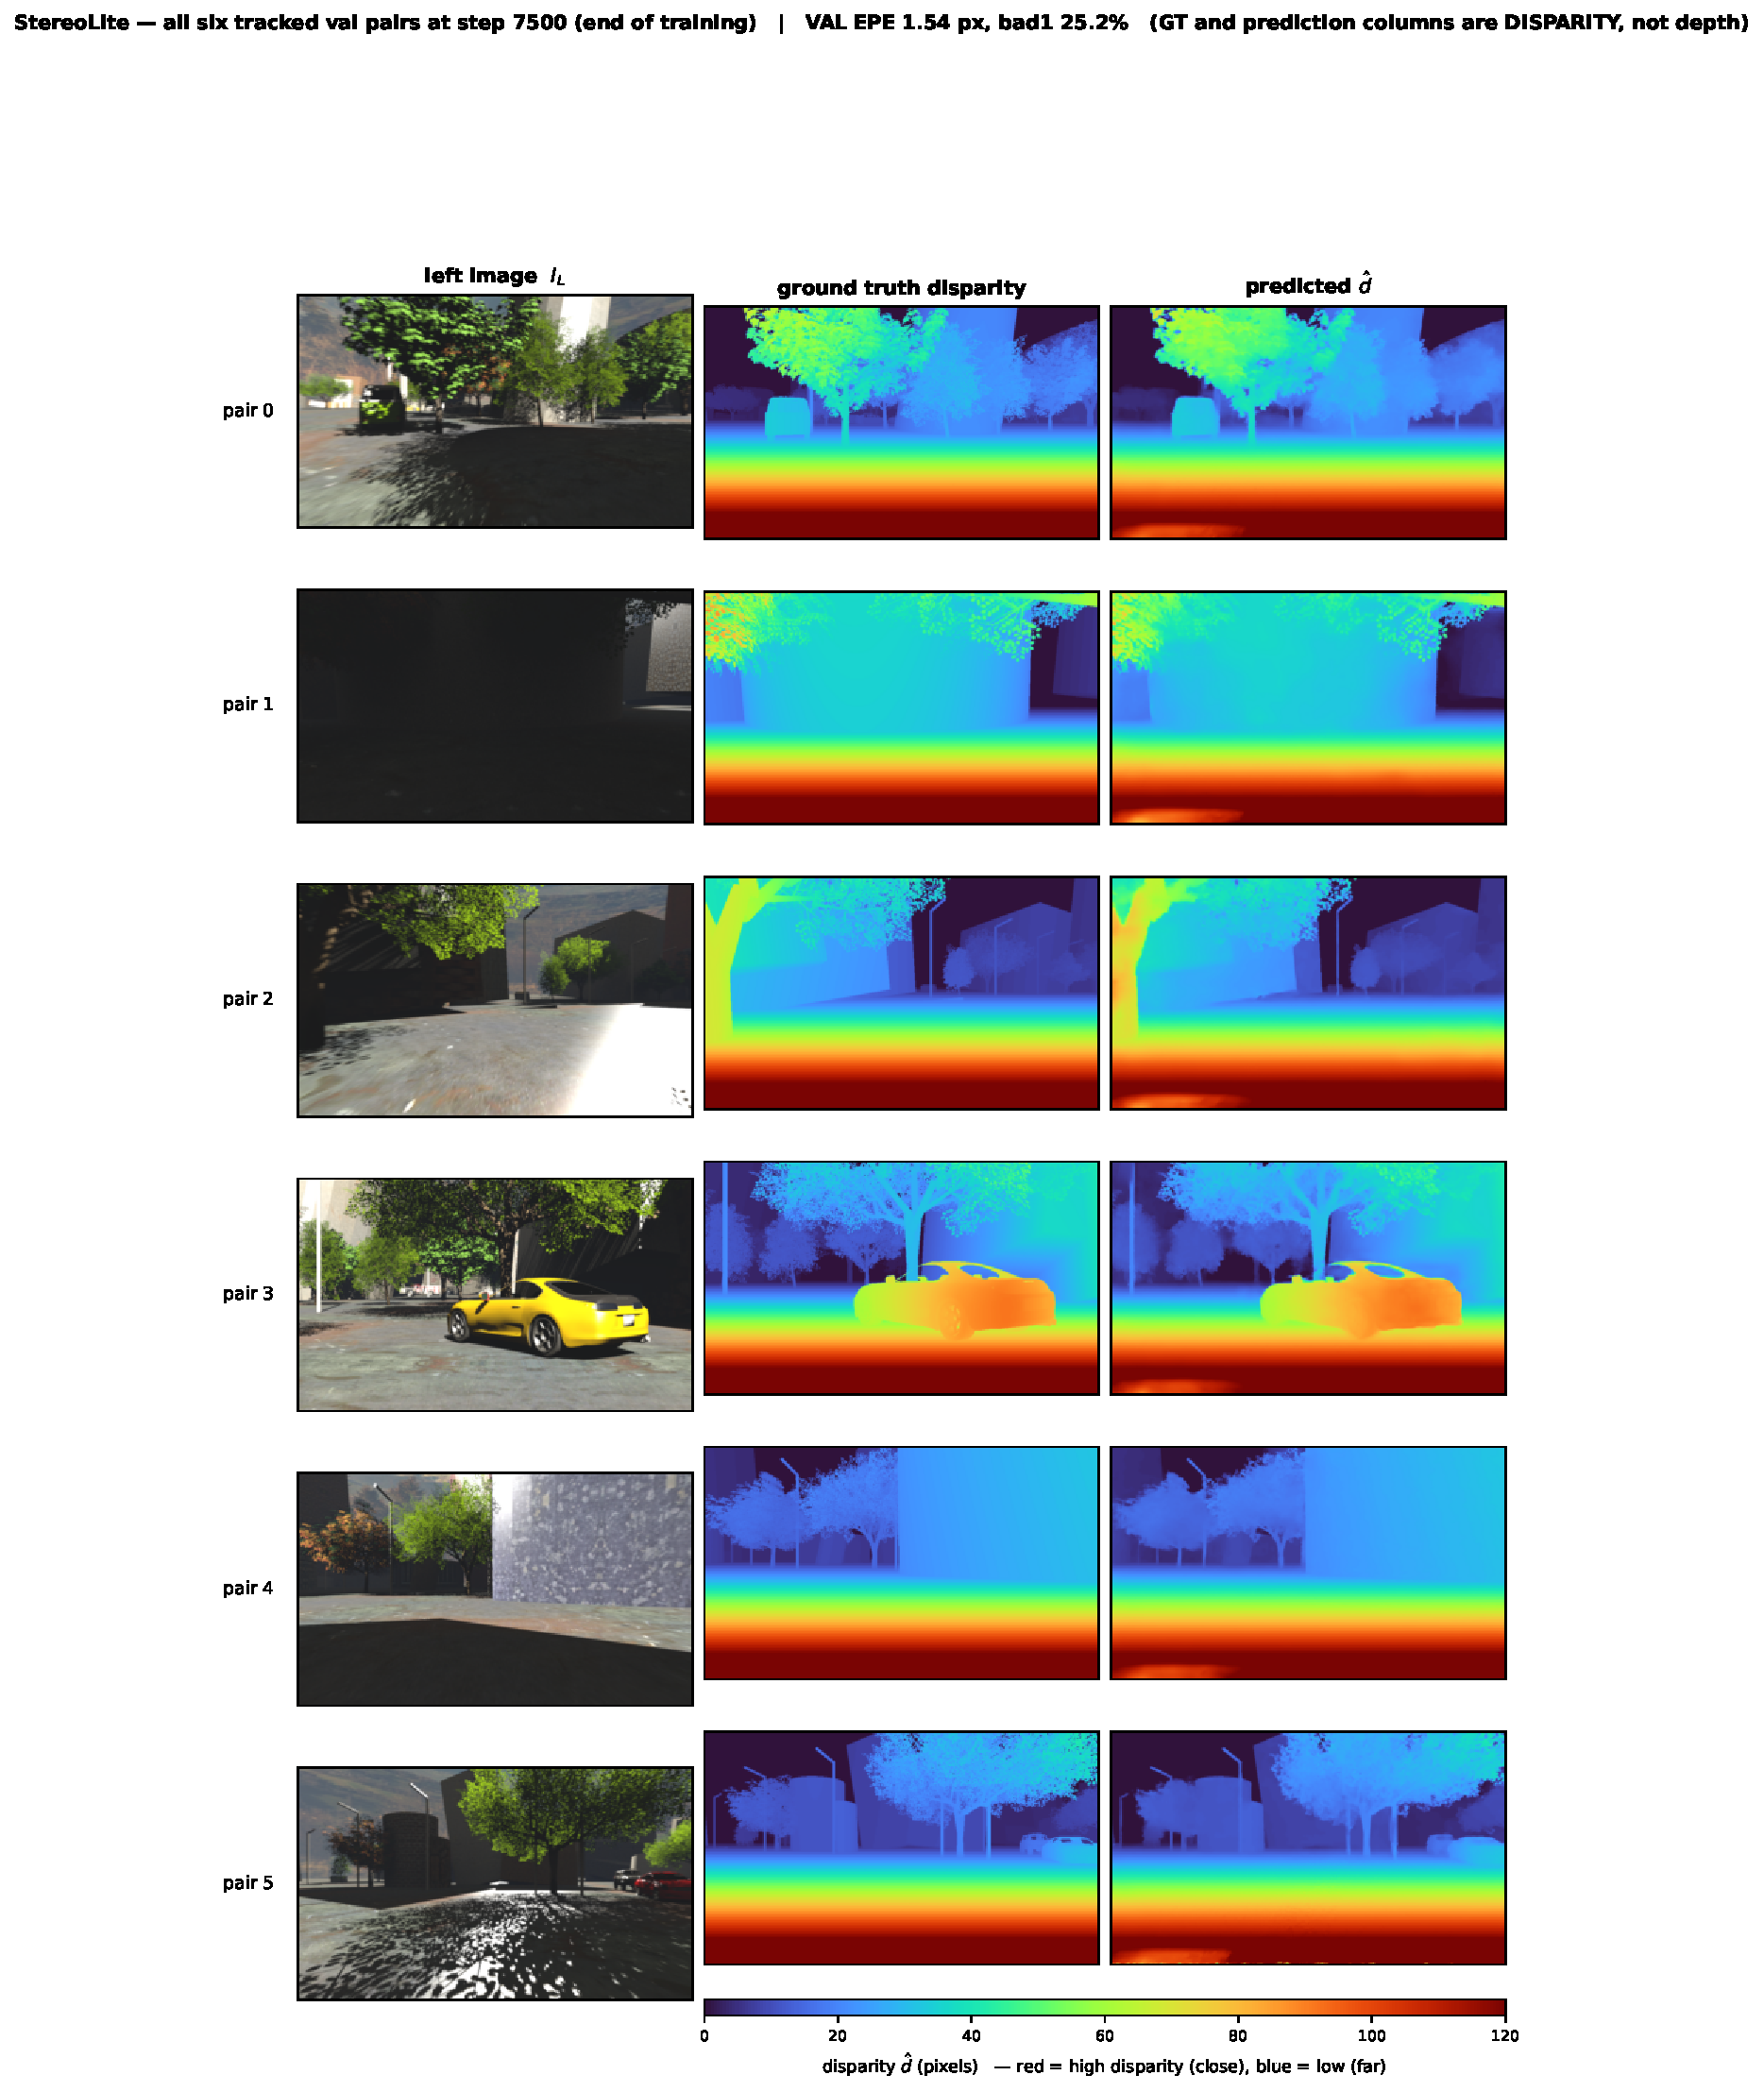
\includegraphics[width=0.92\textwidth]{final_gallery.pdf}
  \caption{All six tracked validation pairs at the final step.
    Columns: left image, ground-truth \textbf{disparity}, predicted
    \textbf{disparity}~$\hat{d}$. TURBO colour map, red = high
    disparity (close), blue = low disparity (far). These are disparity
    maps (pixel shift between left/right views), not depth maps; the
    pinhole conversion to metric depth $Z = f \cdot B / \hat{d}$ is
    applied outside the network.}
  \label{fig:gallery}
\end{figure}

\subsection{Reading the curves and the gallery together}

Two observations worth flagging for review:
\begin{enumerate}[leftmargin=*, topsep=2pt, itemsep=2pt]
  \item The 1/8-scale cost-volume L1 (panel c) drops to about 0.13\,px
    by step~7000 and plateaus. At that scale, 0.13\,px corresponds to
    $\approx$1\,px at full resolution; this gives an effective
    \emph{lower bound} on how accurate the final upsampled disparity
    can be without further architectural changes (a deeper or
    multi-scale cost-volume head would be the next thing to try).
  \item The bad-1 rate of 25\,\% looks high but is dominated by a
    handful of pairs with sparse far-field ground truth (visible in
    pair~1 and pair~5 of Figure~\ref{fig:gallery}). The mean EPE of
    1.54\,px is the more representative number on this dataset.
\end{enumerate}

\subsection{Open items before publication}

\begin{itemize}[leftmargin=*, topsep=1pt, itemsep=1pt]
  \item Pretrain on the full Scene Flow corpus (Driving + Monkaa +
    FlyingThings3D, $\approx$35\,k pairs) instead of Driving only. The
    FlyingThings3D tarballs are downloading via Academic Torrents.
  \item Fine-tune on KITTI 2015 (200 pairs) and report bad-3 on the
    public benchmark.
  \item Cross-domain evaluation on Middlebury 2014 and ETH3D.
  \item INT8 quantisation pass for Jetson Orin Nano deployment;
    measured target $25$--$40$\,ms per pair.
\end{itemize}

\end{document}
